\chapter{TRACE : détection et réduction des hallucinations}
\label{chap:architecture}

\section{Introduction}\label{sec:c5-intro}

Le pipeline du chapitre~\ref{chap:extraction} produit, pour chaque dossier, un graphe d'entités et de relations dont chaque élément est ancré dans le texte de sa page et conforme au schéma. Ces contrôles ne suffisent pas à garantir la fidélité du graphe au dossier. Une entité peut être écrite dans la page et pourtant niée, hypothétique ou relative à un antécédent ; une relation peut respecter le schéma sans que le texte l'énonce ; un même fait peut être répété ou découpé en plusieurs nœuds mal reliés.

Ce chapitre présente TRACE (\textit{Taxonomy and Reduction of hAllucinations in Clinical knowledge Extraction}), la chaîne de vérification construite pour détecter et réduire ces hallucinations après l'extraction. Il définit d'abord la taxonomie des hallucinations sur laquelle elle repose (section~\ref{sec:c5-taxonomie}), puis les principes de son architecture (section~\ref{sec:c5-principes}). Il décrit ensuite chacun de ses étages (sections~\ref{sec:c5-etage1} à~\ref{sec:c5-etage8}), avant de conclure sur ce que la chaîne couvre et sur ses limites (section~\ref{sec:c5-conclusion}). Les résultats sont présentés au chapitre~\ref{chap:experimentations}.

% ------------------------------------------------------------
\section{Taxonomie des hallucinations en extraction clinique multimodale}\label{sec:c5-taxonomie}

Les taxonomies présentées au chapitre~2 ont été construites pour la génération libre de texte~\cite{huang2023survey,ji2023survey} ou pour la description d'images~\cite{bai2025survey}. Dans une tâche d'extraction, la référence n'est pas une connaissance générale du monde mais le document lui-même : une hallucination est un élément du graphe que le dossier ne justifie pas, ou qu'il justifie sous une autre forme. Nous distinguons sept types d'hallucinations, résumés dans la figure~\ref{fig:c5-taxonomie}.

\begin{figure}[H]
\centering
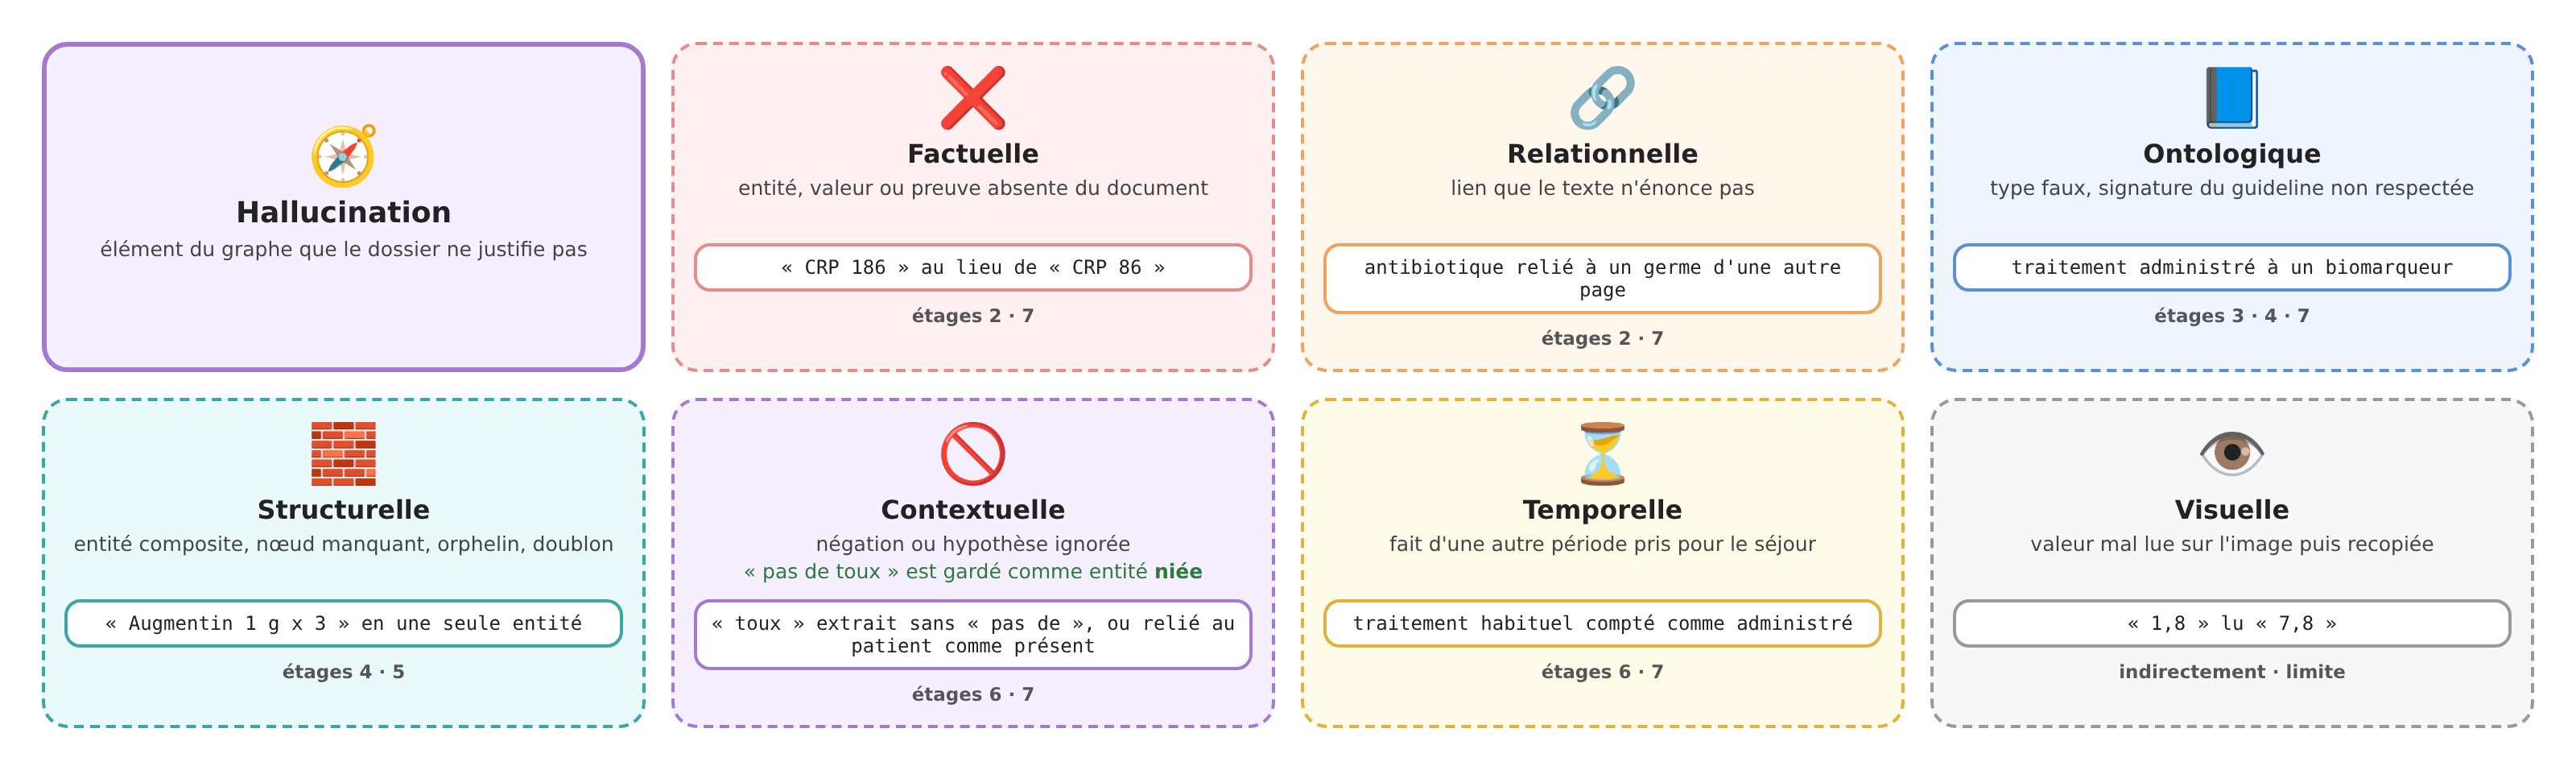
\includegraphics[width=\textwidth]{images/fig_taxonomie_hallucinations.png}
\caption{Taxonomie des hallucinations en extraction clinique multimodale et étages de TRACE qui les traitent (exemples construits pour l'illustration)}\label{fig:c5-taxonomie}
\end{figure}

\begin{itemize}
  \item \textbf{Factuelle} : une entité, une valeur ou une preuve absente du document. C'est la forme la plus directe de l'hallucination, et la plus dangereuse en médecine lorsqu'elle porte sur un chiffre, comme une valeur biologique ou une posologie.
  \item \textbf{Relationnelle} : un lien entre deux entités bien présentes dans le dossier, mais que le texte n'énonce pas. Le modèle déduit la relation de la seule présence des deux entités.
  \item \textbf{Ontologique} : une entité du mauvais type ou une relation qui ne respecte pas les signatures du guideline, par exemple une administration de traitement dirigée vers un biomarqueur.
  \item \textbf{Structurelle} : un graphe mal formé, avec des entités composites qui regroupent deux concepts, des nœuds intermédiaires manquants, des relations orphelines ou des doublons.
  \item \textbf{Contextuelle} : une mention bien écrite dans le texte, mais dont le contexte change le sens, comme une négation ou une hypothèse (\og suspicion de pneumopathie \fg{}). Une absence explicitement mentionnée, comme \og pas de toux \fg{}, n'est pas une hallucination : c'est une information clinique, extraite comme une entité niée, conformément au guideline. L'hallucination consiste à ignorer la négation, en extrayant \og toux \fg{} seul ou en reliant \og pas de toux \fg{} au patient comme un symptôme présent.
  \item \textbf{Temporelle} : un fait d'une autre période pris pour un fait du séjour, par exemple un traitement habituel compté comme administré en réanimation.
  \item \textbf{Visuelle} : une valeur mal lue sur l'image puis recopiée telle quelle dans la transcription, et donc ancrée dans un texte lui-même erroné.
\end{itemize}

Les hallucinations contextuelles et temporelles échappent aux contrôles d'ancrage : le mot \og fièvre \fg{} est bien écrit dans la page. Elles demandent une analyse du contexte de la mention. Les hallucinations visuelles ne sont traitées qu'indirectement, lorsque la valeur mal lue n'est pas cohérente avec le reste du texte ; elles constituent une limite de l'approche.

% ------------------------------------------------------------
\section{Principes de l'architecture}\label{sec:c5-principes}

TRACE est une chaîne d'étages appliquée à la sortie de l'extraction (figure~\ref{fig:c5-architecture}). Sa conception repose sur cinq principes.

\begin{figure}[H]
\centering
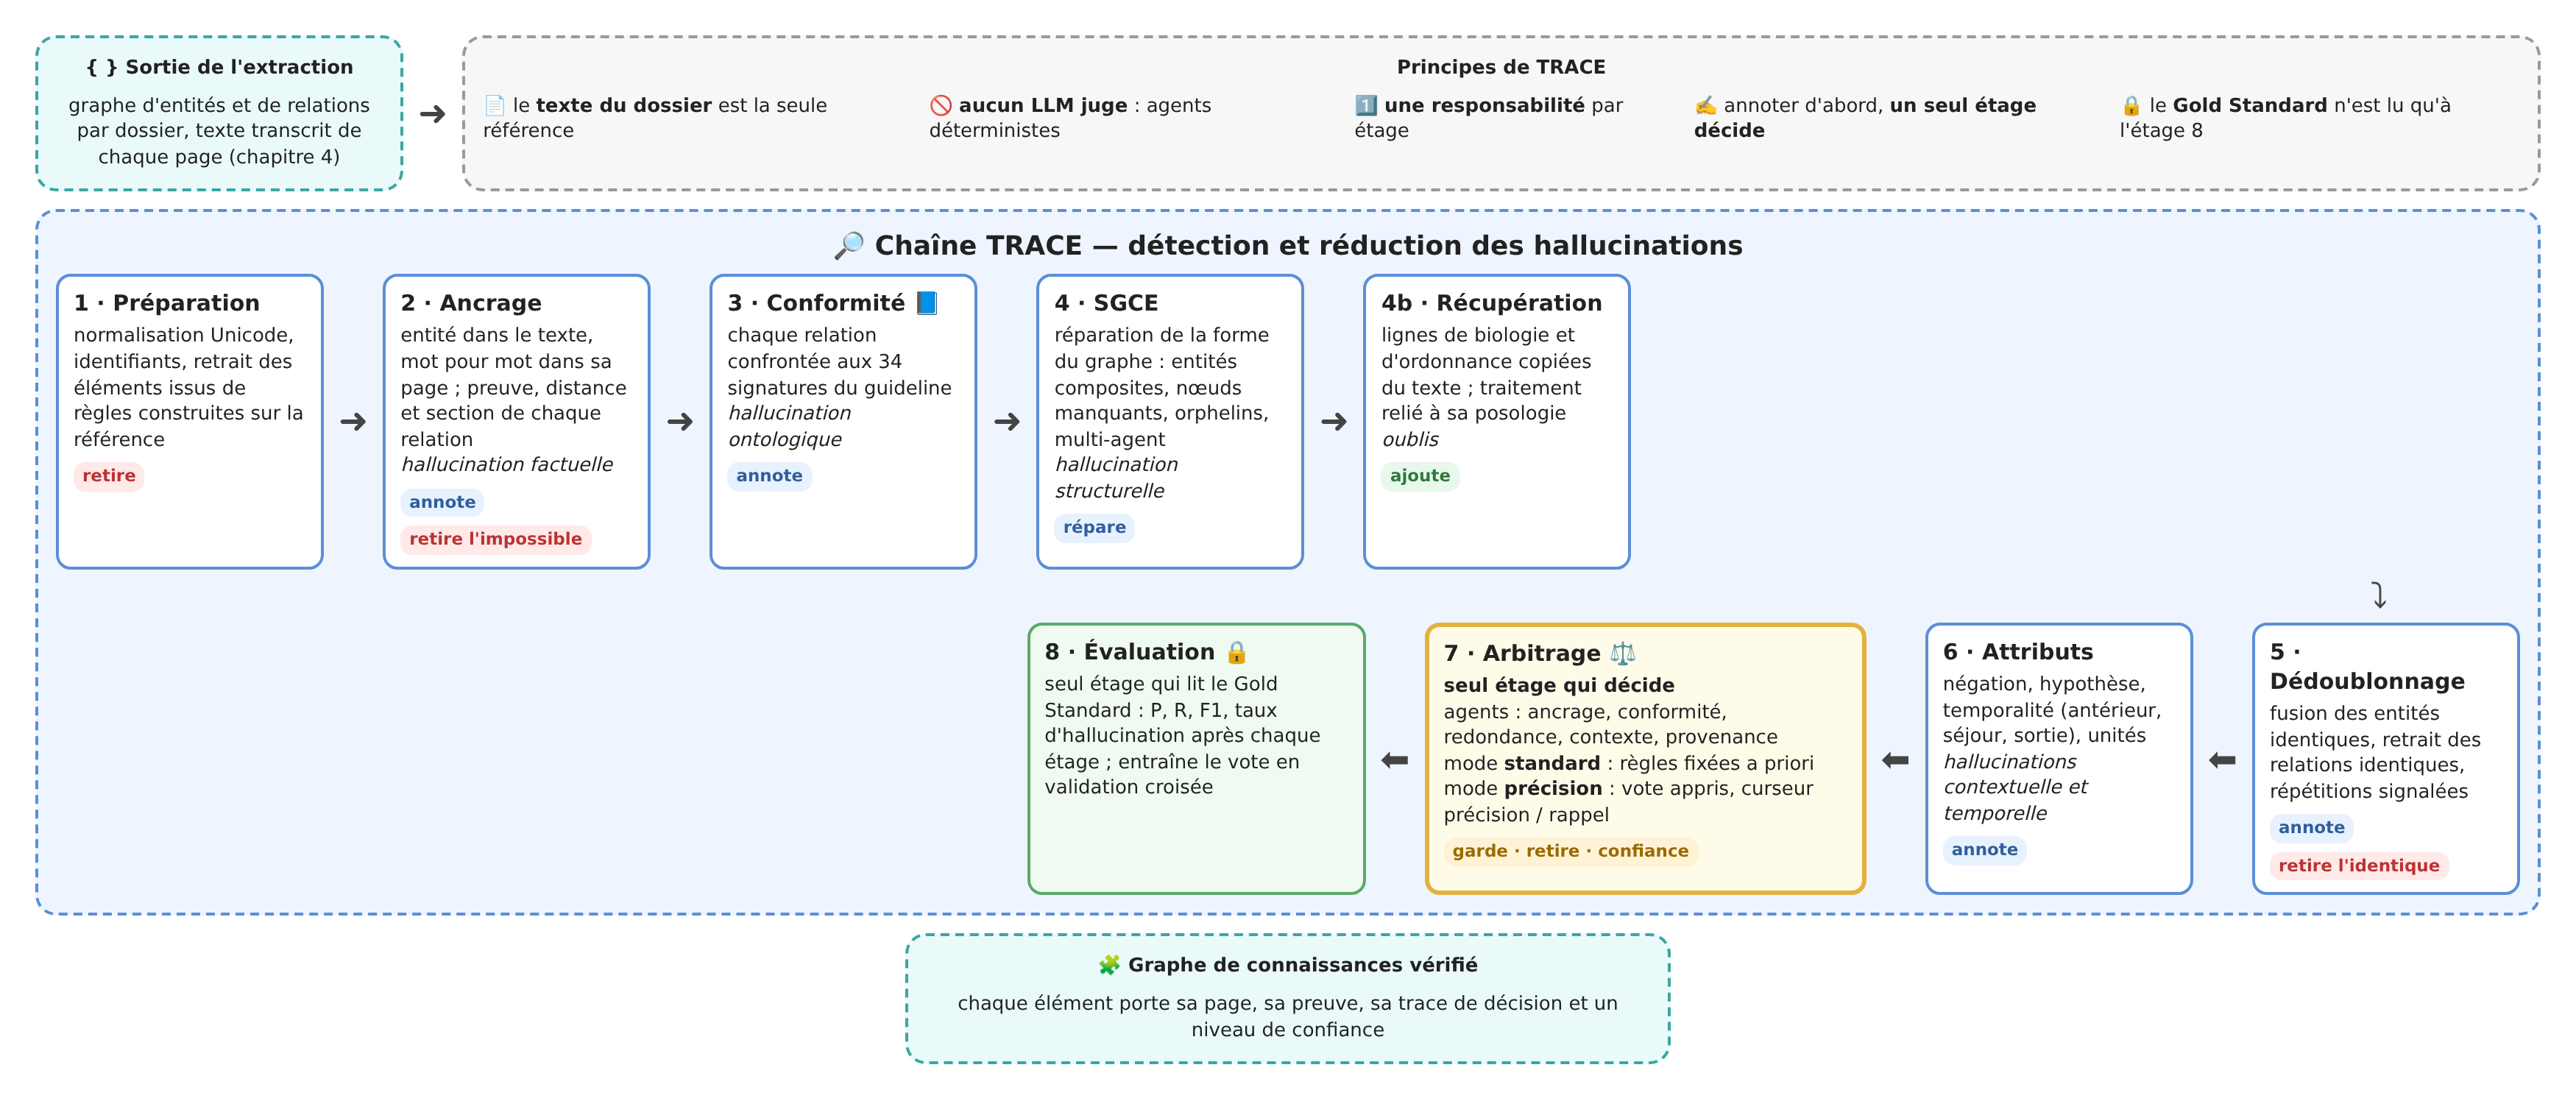
\includegraphics[width=\textwidth]{images/fig_trace_architecture.png}
\caption{Architecture de la chaîne TRACE}\label{fig:c5-architecture}
\end{figure}

\paragraph{Le texte du dossier est la seule référence.} En extraction, l'erreur grave n'est pas une erreur sur une connaissance générale, mais un manque de fidélité au document source~\cite{huang2023survey}. Chaque vérification compare donc l'élément extrait au texte transcrit de sa page, établi une fois pour toutes par le pipeline d'extraction.

\paragraph{Aucun LLM ne sert de juge.} Un grand modèle de langage ne corrige pas de façon fiable ses propres erreurs sans retour extérieur~\cite{huang2024cannot,kamoi2024selfcorrection}, et un modèle juge pourrait lui-même halluciner. Toutes les vérifications de TRACE sont donc déterministes : règles explicites, comparaisons au texte et modèles statistiques simples.

\paragraph{Une seule responsabilité par étage.} Chaque étage traite un seul type de problème. Le gain ou la perte de chaque étage peut ainsi être mesuré séparément, ce qui permet les études d'ablation.

\paragraph{Annoter d'abord, un seul étage décide.} Les étages intermédiaires annotent les éléments sans les retirer, sauf lorsque le document rend l'élément impossible. Un seul étage, l'arbitrage, décide de garder ou de retirer chaque élément, avec toutes les annotations en main. Cette séparation évite les conflits entre étages et les suppressions en cascade incontrôlées.

\paragraph{Le Gold Standard n'est lu que par l'évaluation.} Aucune règle de TRACE n'est réglée sur la référence. Le seul composant appris, le vote du mode précision, est entraîné en validation croisée~\cite{stone1974crossvalidation} : un dossier n'est jamais noté par un modèle qui l'a vu.

Chaque étage écrit ses annotations dans un champ de traçabilité propre à chaque élément. À la sortie de la chaîne, on sait pour tout élément quels étages l'ont examiné, quels signaux ils ont relevés et, s'il a été retiré, quelle règle l'a décidé.

% ------------------------------------------------------------
\section{Étage 1 : préparation}\label{sec:c5-etage1}

Le premier étage rend l'entrée propre et uniforme, sans juger aucun élément. Il retire les éléments qui proviendraient d'un post-traitement construit en regardant la référence, afin que l'évaluation reste valide ; la nouvelle extraction n'en contient pas, mais cette garantie protège la chaîne si elle est appliquée à une sortie plus ancienne. Il met les noms des entités du graphe sous une forme Unicode normalisée (NFKC), de sorte que deux caractères équivalents, comme les deux formes du symbole micro (\og µ \fg{} et \og μ \fg{}), désignent le même nœud. Les mentions des pages restent en revanche telles qu'elles sont écrites dans le texte, puisque l'arbitrage vérifie qu'elles y figurent mot pour mot. Il attribue enfin un identifiant unique à chaque relation qui n'en a pas.

% ------------------------------------------------------------
\section{Étage 2 : ancrage documentaire}\label{sec:c5-etage2}

Le deuxième étage traite les hallucinations factuelles et relationnelles en confrontant chaque élément au texte source.

Pour chaque \textbf{entité}, il vérifie deux propriétés : l'entité est-elle attestée dans le document, c'est-à-dire présente à l'identique ou avec l'essentiel de ses mots et tous ses nombres ? Figure-t-elle mot pour mot dans le texte de sa propre page ? Exiger la présence de tous les nombres répond au risque le plus grave en médecine : une entité \og CRP 186 \fg{} n'est pas attestée si la page indique \og CRP 86 \fg{}.

Pour chaque \textbf{relation}, il relève quatre signaux :
\begin{itemize}
  \item la présence de ses deux extrémités dans le texte ;
  \item le statut de sa \textbf{preuve} : attestée dans le texte, inventée, absente ou simple note du système ;
  \item la \textbf{distance} entre ses deux extrémités : même ligne, même paragraphe, éloignées ou introuvables ; une relation dont une extrémité est le patient n'est pas soumise à cette mesure ;
  \item la \textbf{section} du compte rendu où elle est citée (antécédents, histoire de la maladie, biologie, traitement habituel, sortie\dots).
\end{itemize}

L'étage ne retire que ce que le document rend impossible : une entité absente de tout le texte du dossier, ainsi que les relations qui pointent vers elle ; une relation dont une extrémité n'existe pas dans le texte ; une relation dont la preuve citée n'existe pas ; une relation dont les deux extrémités ne sont jamais à moins de 300~caractères l'une de l'autre. Tout le reste est annoté. Une mention reformulée par le modèle, par exemple une abréviation développée, peut en effet être correcte ; c'est l'arbitrage qui en décide. Ce contrôle correspond à la vérification de fidélité à la source décrite dans la littérature~\cite{ji2023survey}, et à ce que RAPTOR+ appelle les extractions non ancrées~\cite{raptorplus2026}.

% ------------------------------------------------------------
\section{Étage 3 : conformité au guideline}\label{sec:c5-etage3}

Le troisième étage traite les hallucinations ontologiques. Il confronte chaque relation aux 34 signatures du TRACE-Sepsis Annotation Guideline : la relation est-elle autorisée, le type de son sujet correspond-il au domaine attendu, et celui de son objet à l'image attendue ? Chaque relation reçoit le statut conforme, violation de domaine ou violation d'image.

Cet étage annote sans rien retirer, et ce choix est délibéré. Lors de la mise au point de la chaîne, l'examen des relations en violation a montré que la plupart étaient justes : c'est le type d'une de leurs entités qui était faux, non le lien lui-même. Retirer la relation ferait perdre une information correcte, alors que l'étage suivant peut corriger le type de l'entité. La violation devient donc un indice, utilisé par la réparation structurelle et par l'arbitrage. Cette approche rejoint la validation par contraintes des graphes de connaissances~\cite{shacl2017} et les travaux qui combinent LLM et programmation logique~\cite{tran2025aspworkflow}, avec une même réserve : un graphe conforme au schéma n'est pas forcément fidèle au document.

% ------------------------------------------------------------
\section{Étage 4 : réparation structurelle (SGCE)}\label{sec:c5-etage4}

Le quatrième étage traite les hallucinations structurelles avec SGCE (\textit{Structural Grounding for Clinical Knowledge Extraction}), un moteur de réparation développé dans le projet. SGCE applique des motifs d'erreur typés, résumés dans le tableau~\ref{tab:c5-sgce}.

\begin{table}[H]
\centering
\caption{Motifs d'erreur de SGCE et réparations associées}\label{tab:c5-sgce}
\small
\begin{tabular}{p{2.6cm}p{5.4cm}p{5.4cm}}
\toprule
\textbf{Motif} & \textbf{Erreur} & \textbf{Réparation} \\
\midrule
A & entité composite (\og Augmentin 1 g x 3 \fg{}) & découpage en traitement et posologie, reliés entre eux \\
B1 & relation vers une entité absente du graphe & rattachement, ou création de l'entité si le texte la contient \\
B2 & nœud intermédiaire manquant & création du nœud à partir du texte \\
C & lien extrait comme une entité & réécriture en relation \\
D & violation de signature & changement de type ou redirection de la relation \\
Réparation des relations & relation mal typée & correction du type \\
Résolution des orphelins & entité isolée & rattachement au graphe \\
Multi-agent & cas ambigus & vote de plusieurs agents déterministes ; abstention en l'absence de consensus \\
\bottomrule
\end{tabular}
\end{table}

Chaque correction suit un cycle de détection, validation, correction et post-validation : elle n'est conservée que si la structure du graphe s'améliore. Lorsque les agents ne s'accordent pas, SGCE s'abstient plutôt que de corriger au hasard, selon le principe de la décision sélective~\cite{geifman2017selective}. Ses réparations s'inscrivent dans la tradition du raffinement des graphes de connaissances~\cite{paulheim2017refinement} et de la réparation minimale de données sous contraintes~\cite{chu2013holistic,rekatsinas2017holoclean}.

SGCE répare la forme du graphe, non son contenu factuel. Son rôle est de rendre le graphe connexe et conforme au schéma, donc interrogeable, sans dégrader les éléments extraits. Il est utilisé tel quel, dans un espace de travail temporaire, et chaque relation qu'il crée est marquée comme telle afin que l'arbitrage puisse la vérifier à nouveau.

% ------------------------------------------------------------
\section{Étage 4b : récupération structurée}\label{sec:c5-etage4b}

Les étages précédents réduisent les erreurs, mais ne retrouvent pas les éléments que le modèle a oubliés. L'étage~4b ajoute des entités dans les blocs du compte rendu dont la forme est fixe, où le modèle saute souvent des lignes. Il n'invente rien : chaque élément ajouté est un morceau de ligne copié du texte de sa page.
\begin{itemize}
  \item \textbf{B1, biologie} : dans la section de biologie, une ligne de la forme \og libellé, valeur, normes, unité \fg{} (par exemple \og Leucocytes 40.8 4.0-10.0 x10*9/L \fg{}) devient un biomarqueur. Une liste d'exclusion écarte les valeurs témoins du laboratoire et les réglages du ventilateur.
  \item \textbf{B2, ordonnances} : dans les sections de traitement habituel et de sortie, une ligne \og médicament posologie \fg{} (\og Tahor 10mg 0-0-1 \fg{}) donne un traitement et une posologie distincts.
  \item \textbf{B3, posologie} : sur cette même ligne, le traitement est relié à sa posologie par la relation \emph{traitement\_a\_pour\_posologie}, la ligne servant de preuve.
\end{itemize}
Une entité n'est ajoutée que si aucune entité de même type ne la recouvre déjà dans la page, et une relation que si elle n'existe pas déjà. Une quatrième règle, qui reliait chaque traitement d'ordonnance au patient, a été testée puis écartée, car elle ajoutait plus de relations fausses que justes. Ces règles décrivent un format de document et non des réponses de la référence ; elles ont été fixées avant l'évaluation.

% ------------------------------------------------------------
\section{Étage 5 : dédoublonnage}\label{sec:c5-etage5}

Le cinquième étage supprime la redondance sans perdre d'information. Il fusionne les entités strictement identiques (même type, même mention, même page, même valeur, même unité, même négation) et reporte leurs relations sur l'entité conservée. Il retire les relations strictement identiques, c'est-à-dire de même sujet, même type et même objet. Il annote enfin, sans les retirer, les relations qui répètent un triplet déjà vu sous d'autres identifiants. Une telle répétition est souvent une erreur, mais elle peut être légitime, comme une même mesure rapportée deux jours de suite : la décision revient à l'arbitrage.

% ------------------------------------------------------------
\section{Étage 6 : attributs cliniques}\label{sec:c5-etage6}

Le sixième étage traite les hallucinations contextuelles et temporelles. Il qualifie chaque entité, sans rien retirer, selon quatre attributs :
\begin{itemize}
  \item la \textbf{négation} : un mot déclencheur (\og pas de \fg{}, \og absence de \fg{}, \og sans \fg{}, \og aucun \fg{}\dots) précède la mention dans une courte fenêtre, ou l'extraction l'a déjà marquée comme niée ;
  \item l'\textbf{hypothèse} : un indice d'incertitude précède la mention (\og suspicion de \fg{}, \og probable \fg{}, \og à discuter \fg{}\dots) ;
  \item la \textbf{temporalité}, déduite de la section où l'entité est citée : antérieure (antécédents, traitement habituel), de sortie (prescription de sortie) ou du séjour ;
  \item l'\textbf{unité} des valeurs numériques, lorsque la mention contient un nombre suivi d'une unité.
\end{itemize}
La détection de la négation et de l'hypothèse suit le principe de NegEx~\cite{chapman2001negex} et de ConText~\cite{harkema2009context}, adaptés au français~\cite{deleger2012negation} : une liste de déclencheurs et une fenêtre de portée limitée avant la mention. Cette fenêtre couvre \og pas de toux \fg{} sans attraper la négation d'une autre phrase. Sa limite est connue : une expression comme \og arrêt du Lasilix \fg{} ressemble à une négation alors qu'elle décrit un fait réel.

% ------------------------------------------------------------
\section{Étage 7 : agents et arbitrage}\label{sec:c5-etage7}

Le septième étage est le seul qui décide. Pour chaque entité et chaque relation, il choisit de la garder ou de la retirer et attribue un niveau de confiance aux relations. Il s'appuie sur cinq agents déterministes, qui lisent les annotations des étages précédents (figure~\ref{fig:c5-arbitrage}) :
\begin{itemize}
  \item l'\textbf{agent d'ancrage} : preuve, distance entre les extrémités, section (étage~2) ;
  \item l'\textbf{agent de conformité} : respect de la signature du guideline (étage~3) ;
  \item l'\textbf{agent de redondance} : triplet déjà vu sous d'autres identifiants (étage~5) ;
  \item l'\textbf{agent de contexte} : négation, hypothèse et temporalité de l'entité clinique (étage~6) ;
  \item l'\textbf{agent de provenance} : extraction directe par le modèle ou inférence structurelle.
\end{itemize}
Pour une relation créée par SGCE après l'étage~2, les agents appellent les mêmes fonctions de vérification que les étages correspondants.

\begin{figure}[H]
\centering
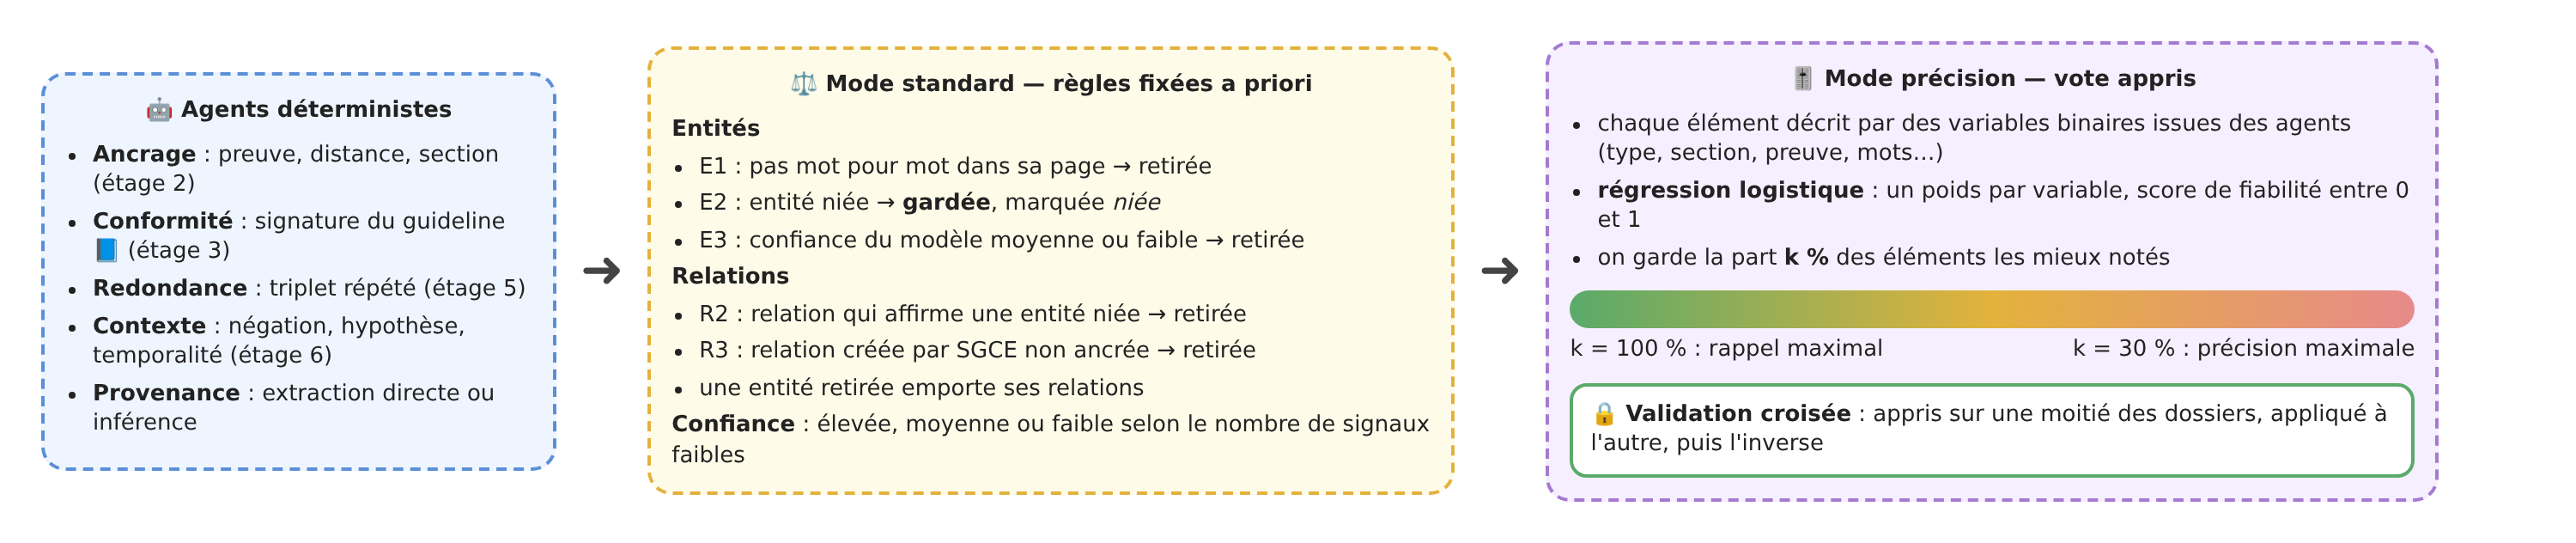
\includegraphics[width=\textwidth]{images/fig_arbitrage.png}
\caption{Arbitrage de l'étage~7 : agents, mode standard et mode précision}\label{fig:c5-arbitrage}
\end{figure}

\subsection{Mode standard : règles fixées a priori}\label{sec:c5-standard}

En mode standard, les décisions suivent des règles fixées avant toute évaluation.

\paragraph{Entités.}
\begin{itemize}
  \item \textbf{E1} : une entité qui ne figure pas mot pour mot dans le texte de sa page est retirée ; c'est une reformulation ou une invention du modèle.
  \item \textbf{E2} : une entité niée (\og pas de toux \fg{}) est \emph{conservée} et marquée comme niée. L'absence d'un signe est une information clinique, et le Gold Standard validé par le médecin l'annote comme telle.
  \item \textbf{E3} : une entité à laquelle le modèle lui-même a attribué une confiance moyenne ou faible est retirée.
\end{itemize}

\paragraph{Relations.}
\begin{itemize}
  \item \textbf{R2} : une relation qui affirme une entité niée (par exemple \og le patient présente le symptôme \emph{pas de toux} \fg{}) est retirée. L'entité niée reste dans le graphe, mais aucune relation ne la donne comme présente, conformément à la convention du guideline.
  \item \textbf{R3} : une relation créée par SGCE qui échoue aux contrôles d'ancrage de l'étage~2 est retirée.
  \item Une entité retirée emporte les relations qui pointent vers elle, afin que le graphe reste cohérent.
\end{itemize}

Une violation de signature n'est pas un motif de retrait, pour la raison donnée à la section~\ref{sec:c5-etage3}. Elle compte parmi les \textbf{signaux faibles} qui déterminent le niveau de confiance d'une relation : preuve non citée, extrémités éloignées, inférence structurelle, doublon, indice de négation ou d'hypothèse, violation de signature non réparée. Une relation sans signal faible reçoit une confiance élevée, avec un signal une confiance moyenne, avec deux signaux ou plus une confiance faible. Ce niveau ne retire rien : il indique au médecin quelles relations vérifier en priorité.

\subsection{Mode précision : vote appris des agents}\label{sec:c5-precision}

Le mode standard ne retire que ce que des règles sûres permettent d'écarter. Le mode précision ajoute un \textbf{vote appris}, qui permet de régler le compromis entre la quantité d'information conservée et sa fiabilité.

Chaque élément est décrit par des variables binaires issues des signaux des agents. Pour une relation : statut de la preuve, distance, section, type de relation, conformité, provenance, temporalité, doublon, négation, hypothèse, ainsi que les mots porteurs de sens de l'entité clinique et des croisements entre ces variables (section et type de relation, type de relation et mot). Pour une entité : type, section, présence d'une relation, longueur de la mention, présence d'un chiffre, provenance, répétition, hypothèse, mots de la mention et leurs croisements avec le type.

Une \textbf{régression logistique}~\cite{cox1958regression}, régularisée, apprend un poids pour chaque variable et fournit un score de fiabilité compris entre 0 et 1. Deux modèles sont appris, un pour les entités et un pour les relations. On conserve ensuite la part $k$ des éléments les mieux notés, parmi ceux que les règles du mode standard n'ont pas déjà retirés. Le paramètre $k$, compris entre 30~\% et 100~\%, agit comme un curseur : une valeur élevée privilégie le rappel, une valeur faible la précision.

Ce choix de modèle répond à trois exigences :
\begin{itemize}
  \item \textbf{l'interprétabilité} : chaque poids a un sens clinique et peut être montré (un biomarqueur cité avec sa valeur dans la section de biologie est fiable, un triplet répété est suspect) ;
  \item \textbf{la frugalité} : le modèle s'apprend sur un petit corpus ;
  \item \textbf{le déterminisme} : il ne peut pas halluciner à son tour.
\end{itemize}
L'agrégation pondérée de signaux imparfaits reprend l'idée de Snorkel~\cite{ratner2017snorkel}, et le choix de ne garder que les éléments les plus sûrs celle de la décision avec rejet~\cite{chow1970reject,geifman2017selective}.

Le vote est le seul composant de TRACE qui apprend de la référence. Il est donc entraîné et évalué en validation croisée à deux plis : les dossiers sont triés puis séparés en rangs pairs et impairs ; le modèle appris sur une moitié note l'autre, puis l'inverse. Ce sont les mêmes plis que ceux des exemples et des règles du pipeline d'extraction (section~\ref{sec:c4-exemples}). Aucun dossier n'est ainsi noté par un modèle qui a vu son annotation.

% ------------------------------------------------------------
\section{Étage 8 : évaluation}\label{sec:c5-etage8}

Le dernier étage est le seul qui lit le Gold Standard. Il compare à la référence la sortie de chaque étage, avec les modes d'appariement et les métriques définis au chapitre~\ref{chap:extraction} (sections~\ref{sec:c4-matching} et~\ref{sec:c4-metriques}). Mesurer après chaque étage montre ce que chacun apporte et vérifie qu'aucun ne dégrade le résultat.

Il entraîne aussi les deux modèles du vote et calcule leurs seuils pour chaque valeur de $k$, puis évalue le mode précision en validation croisée. Il produit enfin des indicateurs de structure qui ne demandent pas la référence : nombre de relations orphelines, de relations identiques et d'éléments absents du texte.

% ------------------------------------------------------------
\section{Conclusion}\label{sec:c5-conclusion}

TRACE organise la réduction des hallucinations en étages spécialisés. Les premiers annotent chaque élément : ancrage dans le texte, conformité au guideline, forme du graphe, répétitions, négation, hypothèse et temporalité. Un étage unique, l'arbitrage, décide ensuite avec toutes ces annotations en main. Ce découpage couvre six des sept types d'hallucinations de la taxonomie, sans recourir à un LLM juge. Chaque décision reste traçable, et le Gold Standard n'intervient que dans l'évaluation et dans le vote appris en validation croisée.

Deux modes répondent à deux usages. Le mode standard applique des règles sûres, fixées a priori. Le mode précision permet de choisir le niveau d'exigence, de l'exploration exhaustive d'un dossier à la construction d'un graphe destiné à l'aide à la décision.

Cette architecture a aussi des limites. Un post-traitement ne peut pas retrouver ce que le modèle n'a jamais extrait, si bien que le rappel reste borné par l'extraction. Les hallucinations visuelles ne sont traitées qu'indirectement, et les erreurs de raisonnement clinique ne sont pas couvertes. Le chapitre suivant mesure l'apport de chaque étage et le compromis du mode précision sur les 49 dossiers du Gold Standard.
